%%%%%%%%%%%%%%%%%%%%%%%%%%%%%%%%%%%%%%%%%%%%%%%%%%%%%%%%%%%%%%%%%%%%%%%%%%%%%%%%
% Classicthesis-Styled CV
% LaTeX Template
% Version 1.0 (22/2/13)
%
% This template has been downloaded from:
% http://www.LaTeXTemplates.com
%
% Original author:
% Alessandro Plasmati
%
% License:
% CC BY-NC-SA 3.0 (http://creativecommons.org/licenses/by-nc-sa/3.0/)
%
%%%%%%%%%%%%%%%%%%%%%%%%%%%%%%%%%%%%%%%%%%%%%%%%%%%%%%%%%%%%%%%%%%%%%%%%%%%%%%%%

%-------------------------------------------------------------------------------
%	PACKAGES AND OTHER DOCUMENT CONFIGURATIONS
%-------------------------------------------------------------------------------

\documentclass[fontsize=14pt,paper=a4]{scrartcl}

\reversemarginpar % Move the margin to the left of the page 

\usepackage[nochapters]{classicthesis}
\usepackage[LabelsAligned]{currvita} % Style for the layout of the document

\usepackage{hyperref}
\usepackage{wrapfig}
\usepackage{graphicx}
\usepackage{color}
\pagenumbering{arabic}
\usepackage{lastpage}

\areaset[current]{390pt}{730pt} % need some extra space

% New command defining the margin text style
\newcommand{\MarginText}[1]{\marginpar{\raggedleft\itshape\footnotesize#1}}

% Basics font styles
\renewcommand{\cvheadingfont}{\Large\color{Black}}
\hypersetup{colorlinks, breaklinks, urlcolor=Blue, linkcolor=Blue}

\newcommand{\ProfileInfo}[2]{\noindent\hangindent=2em\hangafter=0
  \parbox{5em}{\small \textit{#1}\hspace{1em}} {\small #2}}

\newcommand{\WorkEntry}[2]{\noindent\hangindent=2em\hangafter=0%
  {\small #2} {(\small \textit{#1}})\vspace{.5em}}

% Set the width of the date box in each block
\newlength{\datebox}\settowidth{\datebox}{2020---2021}

\date{} % Remove the date at bottom of the documment

\newcommand{\NewEntry}[3]{\noindent\hangindent=2em\hangafter=0%
  \parbox{\datebox}{\small \textit{#1}}\hspace{1em} {\small #2 #3}\vspace{.5em}}

% Define a command for descriptions of each entry - change spacing and font
% sizes here
\newcommand{\Description}[1]{\hangindent=2em\hangafter=0%
  \noindent\raggedright\footnotesize{#1}\par\flushleft\normalsize}

\setlength{\textwidth}{146.8mm}
\setlength{\oddsidemargin}{11.6mm}
\setlength{\evensidemargin}{0.8mm}
% \setlength{\topmargin}{-2.2mm}
% \setlength{\textheight}{221.9mm}
\setlength{\headheight}{14pt}
% Put \marginparwidth onto the page
\setlength{\marginparwidth}{\dimexpr\paperwidth-\oddsidemargin-1in-\textwidth-\marginparsep}

% Footer
\clearpairofpagestyles%
\ihead{\headmark}%
\rofoot*{%
  \makebox[\dimexpr\marginparsep+\marginparwidth\relax]{%
    \thepage\ of \pageref{LastPage}\hfill\rule{.55\marginparwidth}{6pt}%
  }%
}%
% \lofoot*{%
%   \footnotesize LinkedIn: %
%   \href{https://www.linkedin.com/in/matheusvcorrea}{linkedin.com/in/matheusvcorrea}%
% }

\usepackage{tikz}

%-------------------------------------------------------------------------------

\begin{document}

\pagestyle{scrheadings}
% \thispagestyle{empty} % Stop the page count

%-------------------------------------------------------------------------------
%	NAME AND CONTACT INFORMATION SECTION
%-------------------------------------------------------------------------------

\begin{cv}{%
    \noindent%
    \spacedallcaps{%
      MATHEUS V. CORREA%
    }%
    % Header with pic
    % \begin{minipage}{.68\textwidth}%
    %   \spacedallcaps{{\footnotesize R\'ESUM\'E}\\
    %      MATHEUS V. CORREA%
    %   }%
    % \end{minipage}%
    % \hfill%
    % Profile Picture %
    % \begin{minipage}{.30\textwidth}%
    %   \begin{flushright}%
    %     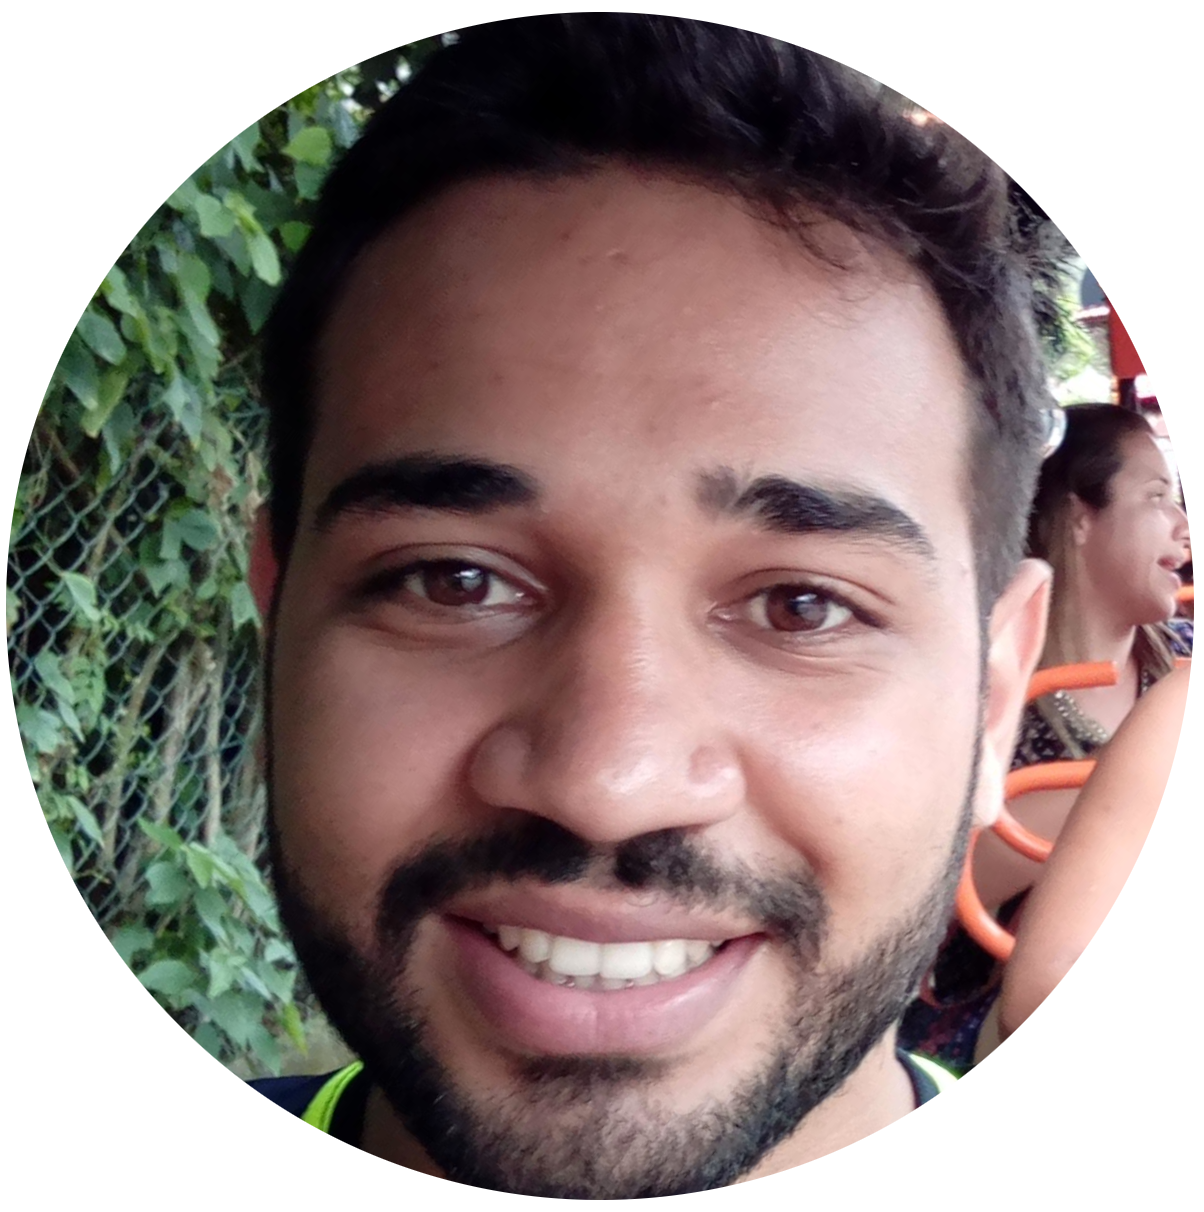
\includegraphics[clip,width=0.6\linewidth]{profile-pic-croped}
    %   \end{flushright}%
    % \end{minipage}%
  } % \vspace{-.7em}
  
  % Goal
  % Birthplace and date
  \noindent{%
    \small\textit{Software Engineer}%
    % $\bullet$ \textit{Looking for sponsorship}%
  }
  
  \vspace{.5em}
  
  % Email address
  \ProfileInfo{email}{\href{mailto:matheusviniciuscorrea@gmail.com}{matheusviniciuscorrea@gmail.com}}

  % Personal website
  \ProfileInfo{LinkedIn}{\href{https://www.linkedin.com/in/matheusvcorrea}{https://www.linkedin.com/in/matheusvcorrea}}

  % Phone number(s)
  % \ProfileInfo{phone}{+353 87 785 5487}
  \ProfileInfo{phone}{+55 11 996174 8484}
  
  \vspace{1em}

  % Goal heading, could be used for a quotation or short profile instead
  \noindent\spacedlowsmallcaps{SUMMARY}\vspace{.5em}
  
  \Description{%
    Master's degree in Informatics at Universidade Federal do Paraná --
    Brazil. With more than 5 years of experience in software development that
    range from e-commerce applications, to distributed systems, and insurance
    risk analysis with machine learning-powered solutions. Strong knowledge in
    C/C++ and Python programming languages. He has knowledge in DDD, TDD, SOLID
    and Design Patterns aside from the main machine learning algorithms and
    frameworks. His main interests are in Algorithms Design, Graph Algorithms,
    Combinatorial Problems, and High Performance Computer Systems. A fan of good
    music, good food, and sports competitions in general.%
  }

%-------------------------------------------------------------------------------
%	WORK EXPERIENCE
%-------------------------------------------------------------------------------

  \noindent\spacedlowsmallcaps{Experience}\vspace{.5em}

  \WorkEntry{Dec. 2020 -- Present}{Back-end Developer at \textsc{Junto Seguros} -- Remote}

  \Description{%
    \MarginText{Junto Seguros}%
    As a back-end developer, he works within the machine learning life cycle
    with an multidisciplinary team at an insurance company. The main
    responsibilities are to contribute to the solution concept and
    implementation phases offering technical/analytical insights under a
    microservices architecture. Different business case applications has been
    created and maintained which include but not limited to credit risk,
    pricing, churn rate, and internal processes automation which combined add
    approximately R\$ 10 mi. in revenue. Moreover he contributes with the
    efforts to keep solutions at state of the art with technology and best
    practices on machine learning powered software with aim to continuous
    improve the ROI ratio. % \newline%
  }

  % ------------------------------------------------

  \WorkEntry{May 2019 -- Jun. 2020}{Senior C++ Programmer at \textsc{Meta} -- Curitiba}
  
  \Description{%
    \MarginText{Meta Serviços de Informática}%
    Worked in different phases of the software development life cycle, mainly in
    the Architecture, Implementation and Testing phases. In the Architecture
    phase he contributes in the definition of business and technical
    solutions. In the Implementation stage, he worked in applications that use
    protocols such as JMS, RPC (XML), SOAP, REST and TCP / IP (Unix Socket). In
    the Testing phase, he worked in automation tests.%
  }

  % ------------------------------------------------

  \WorkEntry{Nov. 2018 -- April 2019}{Programmer at \textsc{Centro Internacional de
      Tecnologia de Software}}

  \Description{%
    \MarginText{C.I.T.S.}%
    Most of his attributions was to programming under the Java EE and Oracle
    Suite (Weblogic, Oracle Data base) to create and support features in legacy
    software.%
  }

  % ------------------------------------------------
  
  \WorkEntry{2018}{Fellow Master's at \textsc{Lactec}}
  
  \Description{%
    \MarginText{Lactec}%
    Main activities: R\&D with regard to optimization problems; studies on
    software and systems engineering; programming on the Java EE, Python, among
    others.%
  }

  % ------------------------------------------------

  % \MarginText{More Experiences}
  
  \WorkEntry{2017}{Intern at Universidade Federal do Paraná}
  
  \WorkEntry{2013}{Freelance E-commerce Developer}
  
%-------------------------------------------------------------------------------
%	EDUCATION
%-------------------------------------------------------------------------------

  \noindent\spacedlowsmallcaps{Education}\vspace{1em}

  \NewEntry{2018 -- 2020}{Universidade Federal do Paraná -- Curitiba}

  \Description{%
    \MarginText{Master's Degree}%
    % Dissertation Title: \textit{Busca em Largura Lexicográfica e Algoritmos
    %   Exatos para o Problema da Clique Máxima}\newline%
    Analytical and experimental research of performance improvements made using
    the so called lexicographic breadth-first search on algorithms that solve
    the maximum clique problem, a well know hard to compute graph
    problem. Related English publication available at
    \url{http://doi.org/10.21711/231766362021/rmc4824}\newline%
    Advisors: Prof.~Dr.~Renato \textsc{Carmo} \& Prof.~Dr.~Alexandre
    \textsc{Z\"uge}%
  }
  
  % ------------------------------------------------

  \NewEntry{2014 -- 2017}{Universidade Federal do Paraná, Campus Jandaia do Sul}

  \Description{%
    \MarginText{Bachelor's Degree}%
    % Monograph Title: \textit{Técnicas de Projeto de Algoritmos: Backtracking e
    %   Programação Dinâmica.}\newline%
    This degree course gives permission to teach Computer Science. During the
    course he has collaborated in research projects in classical computer
    science subjects such as Sort Algorithms, Graphs Algorithms, Data Structure,
    and Algorithm Design.\newline%
    Monograph published at \url{https://hdl.handle.net/1884/56255}\newline%
    Advisor: Prof.~Dr.~Alexandre \textsc{Z\"uge}%
  }

  % ------------------------------------------------

  \NewEntry{2021 -- 2021}{Graduate Special Student at Unicamp, IC -- Campinas}
  
  % \Description{%
  %   \MarginText{Graduate Special Student}%
  %   Description: As a graduate special student at Instituto de Computação
  %   Graduate Program he attended to classes such Parallel Programming,
  %   Supervised Learning, and Approximation Algorithms.%
  % }

  \vspace{1em}

%-------------------------------------------------------------------------------
%	PUBLICATIONS
%-------------------------------------------------------------------------------

  % \noindent\spacedlowsmallcaps{Publications}\vspace{1em}

  % \NewEntry{January 2022}{Lexicographic Breadth First-Search and Branch and
  %   Bound Algorithms for the Maximum Clique Problem}

  % \Description{%
  %   \MarginText{Matemática Contemporânea}%
  %   We perform an experimental analysis on five branch and bound algorithms for
  %   the Maximum Clique problem. The analysis is done through the usual
  %   statistical hypothesis testing framework. The method shows itself powerful
  %   in discriminating the cases where a new implemented heuristic is effective
  %   and those where it is not.
  %   \url{http://doi.org/10.21711/231766362021/rmc4824}\newline%
  %   Authors: Matheus \textsc{Correa}, ~Renato \textsc{Carmo}, ~Alexandre Prusch
  %   \textsc{Z\"uge}%
  % }

%-------------------------------------------------------------------------------
%	COMPUTER SKILLS
%-------------------------------------------------------------------------------

  % \spacedlowsmallcaps{Computer Skills}\vspace{1em}

  % \Description{\MarginText{Basic}\textsc{java}, Adobe Illustrator}

  % \Description{\MarginText{Intermediate}\textsc{python}, \textsc{html}, \LaTeX,
  %   OpenOffice, Linux, Microsoft Windows}

  % \Description{\MarginText{Advanced}Computer Hardware and Support}

  % \vspace{.5em} % Extra space between major sections

%-------------------------------------------------------------------------------
%	OTHER INFORMATION
%-------------------------------------------------------------------------------

  \spacedlowsmallcaps{Other Information}\vspace{1em}

  % Create a new length for the length of languages to keep them equally spaced
  \newlength{\langbox}

  % Length equals the length of "English" - if you have a longer language in
  % your list put it here
  \settowidth{\langbox}{English}

  \vspace{-0.5em}
  \Description{%
    \MarginText{Languages}%
    \parbox{\langbox}{\textsc{English}}\hspace{.5em} ---\ \ Can write and speak
    fluently%
  }

  \vspace{-0.5em}
  \Description{%
    \parbox{\langbox}{\textsc{Spanish}}\hspace{.5em} ---\ \ Can communicate with
    simple words and phrases%
  }

  \vspace{-0.5em}
  \Description{%
    \parbox{\langbox}{\textsc{Portuguese}}\hspace{.5em} ---\ \ Mother tongue%
  }

  \vspace{1em}

  % ------------------------------------------------

  \Description{%
    \MarginText{Hobbies and Interests}%
    Football (soccer)\ \ $\cdot$\ \ Instruments\ \ $\cdotp$\ \ Food and beer\ \
    $\cdotp$\ \ Running and workout\ \ $\cdotp$\ \ Movies\ \ $\cdotp$\ \ Funny
    scientific facts \ \ $\cdotp$\ \ Sports competitions in general%
  }

\end{cv}

\end{document}
